%compile with lualatex

\documentclass[a4paper,11pt,abstracton]{scrartcl}

% \input{header}
\usepackage[top=2.5cm,left=2.7cm,right=2.7cm,bottom=2.5cm]{geometry}

\usepackage{xcolor}
\definecolor{f1}{HTML}{E41A1C}

% \addtokomafont{section}{\color{f1}}
% \addtokomafont{subsection}{\color{f1}}
% \addtokomafont{subsubsection}{\color{f1}}
% \addtokomafont{paragraph}{\color{f1}}

\usepackage{rotating}
% \usepackage{mathabx}
\usepackage{lmodern}
% \usepackage{microtype}
\usepackage{amssymb}
\usepackage{amsmath}

\usepackage[T1]{fontenc}
\usepackage{fontspec}
\usepackage{polyglossia}
\setdefaultlanguage[spelling=new, babelshorthands=true]{german}

\usepackage{libertine}

\usepackage{textcomp}
\usepackage{booktabs}

\usepackage[object=vectorian]{pgfornament}
% \usepackage{psfrag}
\usepackage{graphics}
\usepackage{color}
\usepackage[squaren]{SIunits}

\setlength{\textheight}{227mm}
\setlength{\voffset}{0.75cm}

\def\hksqrt{\mathpalette\DHLhksqrt}
\def\DHLhksqrt#1#2{\setbox0=\hbox{$#1\sqrt{#2\,}$}\dimen0=\ht0
\advance\dimen0-0.2\ht0
\setbox2=\hbox{\vrule height\ht0 depth -\dimen0}%
{\box0\lower0.4pt\box2}}

\newcommand{\vektor}[1]{\mathbf{#1}}
\newcommand{\HRule}{\rule{\linewidth}{0.5mm}}
\newcommand{\Folge}[1]{(#1_n)_{n \in \mathbb{N}}}
\newcommand{\gms}[2]{[#1,#2]}

\interfootnotelinepenalty=10000

 \renewcommand{\labelenumi}{(\arabic{enumi})}

\begin{document} %\onehalfspacing
\section{Ordnungen}
Unter Ordnungen (oder Relationen) verstehen wir Relationen, die jeweils zwischen zwei Elementen einer Grundmenge $X$ bestehen oder nicht bestehen. Technisch kann man dafür schreiben, dass die Relation eine Funktion des Typs $X \times X \to \{ \mathrm{wahr}, \mathrm{falsch}\}$ ist. Die Menge $X$ ist der Gegenstandsbereich der Betrachtungen und kann sehr vieles sein; bspw. endlich oder unendlich groß. Für das Bestehen einer Relation $\equiv$ zwischen zwei Gegenständen $x,y \in X$ schreibt man statt $\equiv (x,y) = \mathrm{wahr}$ auch $x \equiv y$ (wie z.B. bei $+$).

Gewisse Ordnungen sind besonders interessant, da sie gewissen Regeln gehorchen. Daher führt man die folgenden Begriffe ein:
\paragraph{Definition (reflexive Relation)} Eine Relation $\leq$ auf $X$ heißt reflexiv, falls für alle $x \in X$
\begin{equation}
 x \leq x.
\end{equation}
\paragraph{Definition (symmetrische Relation)} Eine Relation $\equiv$ auf $X$ heißt symmetrisch, falls für alle $x,y \in X$
\begin{equation}
 x \equiv y \quad \Rightarrow \quad y \equiv x.
\end{equation}
\paragraph{Definition (antisymmetrische Relation)} Eine Relation $\leq$ auf $X$ heißt antisymmetrisch, falls für alle $x,y \in X$
\begin{equation}
 (x \leq y \quad \textnormal{ und } \quad y \leq x) \quad \Rightarrow \quad x = y.
\end{equation}
\paragraph{Definition (transitive Relation)} Eine Relation $\leq$ auf $X$ heißt transitiv, falls für alle $x,y,z \in X$
\begin{equation}
 (x \leq y \quad \textnormal{ und } \quad y \leq z) \quad \Rightarrow \quad x \leq z.
\end{equation}
\paragraph{Definition (totale Relation)} Eine Relation $\leq$ auf $X$ heißt total, falls für alle $x,y \in X$
\begin{equation}
 x \leq y \quad \textnormal{ oder } \quad y \leq x.
\end{equation}
\paragraph{Beispiele} Illustrieren wir dies durch ein paar Beispiele:
\begin{enumerate}
 \item Eine sehr einfache Relation auf allen Mengen $X$ ist die der Identität, $=$. Betrachte z.B. $X = \{1,2,3\}$ oder $X = \mathbb{N}$ oder $X= \{ \textnormal{Peter}, \textnormal{Paul}, \textnormal{Marie} \}$. Die Identität ist reflexiv, symmetrisch und transitiv.
 \item Auf der Menge $\mathbb{N}$ gibt es eine Relation $x$ ist kleiner gleich $y$. Diese Relation ist reflexiv, antisymmetrisch und transitiv und total. Aufgabe: Wie sieht es bei kleiner aus? Wie bei der Nachfolger-relation ``$y$ ist Nachfolger von $x$, oder $y = x +1$''?
 \item Eine Relation, die so ähnlich wie die Identität ist, ist die gleichen Rests bei Division durch 7 auf $\mathbb{Z}$, oder $x \sim y :\Leftrightarrow \exists n \in \mathbb{Z} \ x = y + 7n$. Sie ist reflexiv, symmetrisch und transitiv.
 \item Die Liebes-Relation (von wikipedia), ``$x$ liebt $y$'':
 \begin{center}
  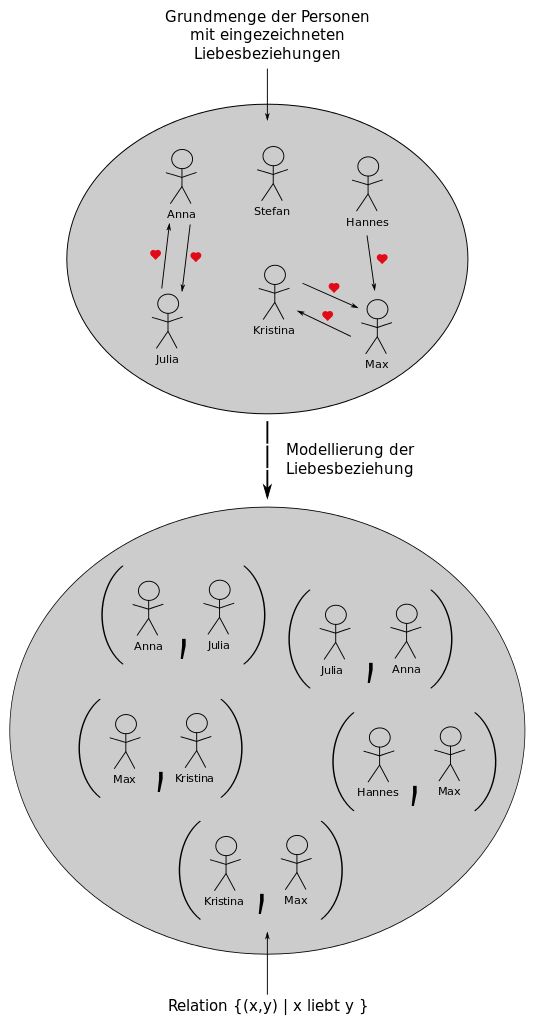
\includegraphics[width=5cm]{liebesrelation}
 \end{center}
\end{enumerate}

Aufgabe: Welche Relationen gibt es auf einer zweielementigen Menge wie $X=\{1,2\}$? Welche davon erfüllen welche der definierten Eigenschaften? Wie viele Relationen gibt es auf $X=\{1,2,3\}$?

Zusammenfassend definiert man
\paragraph{Definition (Äquivalenzrelation)} Eine Relation auf $X$ heißt Äquivalenzrelation, falls sie reflexiv, symmetrisch und transitiv ist.
\paragraph{Definition (Halbordnung)} Eine Relation auf $X$ heißt Halbordnung, falls sie reflexiv, antisymmetrisch und transitiv ist.
\paragraph{Definition (Totalordnung)} Eine Relation auf $X$ heißt Totalordnung, falls sie Halbordnung und total ist.
\paragraph{Beispiele}
\begin{enumerate}
 \item Die Relation $\leq$ auf den natürlichen Zahlen $\mathbb{N}$ ist eine Totalordnung.
 \item Auf der Menge der Paare der natürlichen Zahlen $\mathbb{N} \times \mathbb{N}$, können wir definieren:
 \begin{equation}
  (n_1, m_1) \leq (n_2, m_2) \quad :\Leftrightarrow \quad (n_1 \leq n_2) \quad \textnormal{und} \quad (m_1 \leq m_2)
 \end{equation}
 Die Relation ist dann nur noch eine Halbordnung.
 \item Auf der Potenzmenge der natürlichen Zahlen $\mathcal{P}(\mathbb{N})$ können wir die Teilmengenrelation betrachten. Welche Eigenschaften hat sie?
 \item Aufgabe: Finde ein Beispiel für eine Totalordnung auf $\{1,2,3\}$ und ein Beispiel für eine Halbordnung, die keine Totalordnung ist.
\end{enumerate}
Hat man eine Grundmenge $X$ zusammen mit einer Teilmenge $Y \subseteq X$ gegeben, kann man eine Relation $R$ auf $X$ einschränken zu einer Relation auf $Y$, schreibe $R \upharpoonright Y$.
\paragraph{Lemma} Falls eine Relation $R$ auf $X$ reflexiv, symmetrisch, antisymmetrisch, transitiv oder total ist, so ist $R\upharpoonright Y$ dies auf $Y$.

Zu einer Relation $R$ (nicht unbedingt transitiv) können wir ihren transitiven Abschluss $R^+$ definieren:
\begin{equation}
 x R^+ y \quad :\Leftrightarrow \quad \exists n \geq 0 \quad \exists x_1, \dots, x_n \textnormal{ mit } x R x_1 \textnormal{ und } x_1 R x_2 \textnormal{ und } \dots \textnormal{ und } x_n R y
\end{equation}
\paragraph{Lemma} Der transitive Abschluss $R^+$ ist transitiv.
\paragraph{Aufgabe} Für eine transitive Relation $R$ ist $R^+ = R$, oder $x R y \Leftrightarrow x R^+ y$.
\paragraph{Aufgabe} Es gilt ${R^+}^+ = R^+$.
\subsection{Über Äquivalenzrelationen}
Hat man auf einer Menge $X$ eine Äquivalenzrelation $\sim$ gegeben, so induziert diese folgende interessante Menge, die häufig Menge der Äquivalenzklassen genannt wird.
\begin{equation}
 X / \sim \quad := \quad \{ [x] \, | \, x \in X \}, \quad \textnormal{wobei} \quad [x] = \{ y \in X \, | \, x \sim y\}
\end{equation}
Zum Beispiel ist dann $\{[0], [1], \dots, [6] \}$ die Menge der Äquivalenzklassen von $\mathbb{Z}$ bezüglich der Teilbarkeitsrelation, mit $[0] = \{ \dots, -14, -7, 0, 7, 14, \dots \}$.

Wir können zu dem Element $n$ aus $\mathbb{Z}$ einen eindeutigen Repräsentanten wählen, z.B. die Zahl zwischen 0 und 6, die zu $n$ äquivalent ist. Damit bekommen wir aus der totalen Ordnung $\leq$ auf $\mathbb{Z}$ auch eine Ordnung auf $\mathbb{Z}/ \sim$. Diese ,,Vererbung'' von Eigenschaften oder Funktionen ist ein mächtiges Werkzeug.
\subsection{Über Halb-Ordnungsrelationen}
Halbordnungsrelationen können durch sogenannte Hasse-Diagramme dargestellt werden. Dabei werden die Elemente von $X$ durch Punkte dargestellt. Beipiele: $B_3$, $B_4$, endliche totale geordnete Mengen. Die Idee ist, dass Pfeile von Punkten zu sich selber weggelassen werden können, weil die Relation eh reflexiv ist. Ähnliches gilt für Transitivität. Die Richtung der Ordnung wird durch die Höhe im Bild dargestellt.

\paragraph{Lemma} $B_3$ und $B_4$ sind Halbordnungen.

Haben wir eine Menge $X$ und eine Halbordnungsrelationen $\leq$ gegeben, sowie $Y \subseteq X$ und $x \in X$. Dann definieren wir
\paragraph{Definition (obere Schranke)} $x$ ist eine obere Schranke von $Y$, falls für alle $y \in Y$ $y \leq x$. Schreibe auch $x \gtrsim X$.
\paragraph{Definition (untere Schranke)} $x$ ist eine untere Schranke von $Y$, falls für alle $y \in Y$ $x \leq y$. Schreibe auch $x \lesssim X$.
\paragraph{Definition (Supremum)} Ein $x$ heißt Supremum von $Y$ als Teilmenge von $X$, falls
\begin{enumerate}
 \item $x \in X$,
 \item $x \gtrsim Y$ und
 \item für alle oberen Schranken $y \in X, y \gtrsim Y$ ist $x \leq y$. (Man sagt auch: $x$ ist die kleinste obere Schranke.)
\end{enumerate} Schreibe auch $x = \bigvee Y$.

Nach unten definiert man analog das Infimum, schreibe auch $\bigwedge Y$.

\paragraph{Definition (Verband)} Ein $X$ heißt Verband, falls jede nicht-leere endliche Teilmenge $Y \subseteq X$ ein Supremum und ein Infimum hat.
\paragraph{Definition (vollständiger Verband)} Ein $X$ heißt vollständiger Verband, falls jede Teilmenge ein Supremum und ein Infimum hat.
\paragraph{Lemma} Ein $X$ ist vollständiger Verband genau dann, wenn bereits jede Teilmenge ein Supremum (Infimum) hat.
\paragraph{Beispiele} In $B_3$ ist $t$ das Supremum der Menge $\{t,f,\}$ und $n$ das Infimum. Aber die Menge $\{t,f\}$ hat bloß ein Infimum, $n$, aber kein Supremum (denn keine obere Schranke) in $B_3$. In $B_4$ ist aber das Supremum $b_4$. Da auch alle anderen Teilmengen ein Supremum und Infimum haben, ist $B_4$ also ein vollständiger Verband.
\section{Ccpos}
$B_3$ erfüllt allerdings ein anderes Kriterium, das man in folgender Definition zusammenfasst:
\paragraph{Definition (Konsitenz)} Eine Mengen $Y \subseteq X$ heißt konsistent auf $X$ Halbordnung, falls jede Menge $\{u,v\} \subseteq Y$ eine obere Schranke in $X$ hat.
\paragraph{Definition (Ccpo)} Ein $X$ heißt Ccpo, falls jede konsistente Teilmenge ein Supremum hat.
\paragraph{Lemma} Die leere Menge und alle einelementigen Menge sind konsistent.
\paragraph{Beispiele} Die konsistenten Teilmengen von $B_3$ sind $\varnothing, \{ t\}, \{f \}, \{n\}, \{n,t\}, \{n,f\}$.

In $B_4$ sind alle Teilmengen konsistent, weil
\paragraph{Lemma} In einem vollständigen Verband sind alle Mengen konsistent.

\paragraph{Weitere Beispiele} Ccpos und nicht-ccpos gemäß Gupta Belnap.

Ccpos haben viele hilfreiche Eigenschaften:
\paragraph{Theorem über Ccpos (Teil I)} Sei $X$ mit $\leq$ eine Ccpo, und sei $x \in X$. Dann gilt
\begin{enumerate}
 \item[(i)] $X$ hat ein kleinstes Element, d.h. es gibt $\perp \in X$ mit $\perp \lesssim X$.
 \item[(ii)] Jede nicht-leere Teilmenge von $X$ hat ein Infimum.
\end{enumerate}
\paragraph{Beweis} Zu (i): Die leere Menge ist konsistent, also gibt es $\perp = \bigvee \varnothing$. Nun zeigen wir $\perp \lesssim X$, d.h. $\perp \leq x$ für alle $x \in X$. Sei $x \in X$ beliebig. Dann ist $x \gtrsim \varnothing$, da dafür nichts zu zeigen ist, und also $\perp \leq x$, weil $\perp$ Supremum der leeren Menge war.

Zu (ii): Sei $Y \subseteq X$ nicht-leer. Betrachte dann $Z := \{ u \in X \, | \, u \lesssim Y\}$.

Zuerst zeigen wir, dass $Z$ konsitent ist. Seien $u,v\in Z$ gegeben, also $u \lesssim Y$ und $v \lesssim Y$. Da es mindestens ein Element von $Y$ gibt, sagen wir $\hat y$, folgt $u \leq \hat y$ und $v \leq \hat y$. Das bedeutet aber, dass $\hat y$ eine obere Schranke für $u$ und $v$ ist.

Da $X$ ccpo war, gibt es also ein Supremum von $Z$, $\bigvee Z$. Wir zeigen nun, dass dies ein Infimum von $Y$ ist.

Zuerst müssen wir zeigen, dass $\bigvee Z \lesssim Y$, oder für ein beliebiges $y \in Y$ gilt $\bigvee Z \leq y$. Irgendein $y \in Y$ ist aber obere Schranke zu $Z$, also $\bigvee Z \leq y$ wie benötigt.

Anders herum liegt jede untere Schranke $z$ zu $Y$ bereits in $Z$, also ist $z \leq \bigvee Z$.
\paragraph{Theorem über Ccpos (Teil II)} Sei $X$ mit $\leq$ eine Ccpo, und sei $x \in X$. Dann gilt
\begin{enumerate}
 \item[(iii)] Falls $X$ ein größtes Element hat, so ist es ein vollständiger Verband.
 \item[(iv)] Die Menge $Y := \{ y \in X \, | \, x \leq y\}$ ist eine ccpo mit $\leq \upharpoonright Y$ als Ordnung.
 \item[(v)] Die Menge $Z := \{ z \in X \, | \, z \leq x\}$ ist ein vollständiger Verband mit $\leq \upharpoonright Z$ als Ordnung.
\end{enumerate}
\paragraph{Beweis} Zu (iii) und (v): Übung!

Zu (iv): Eine konsistente Teilmenge $U \subseteq Y$ ist auch konsistent in $X$, da die obere Schranke aus $Y$ auch in $X$ liegt. Also hat $U$ ein Supremum $u$ in $X$. Falls $U = \varnothing$, so ist $x$ als minimales Element Supremum von $U$. Falls $U \neq \varnothing$ ist $u$ auch das Supremum in $Y$. Denn das Element in $U$ stellt zusammen mit der Transitivität sicher, dass $x \leq u$.

\paragraph{Theorem über Ccpos (Teil III)} Sei $X$ mit $\leq$ eine Ccpo, und sei $x \in X$. Dann gilt
\begin{enumerate}
 \item[(vi)] Es gibt ein maximales Element von $X$ größer oder gleich $x$, d.h. es gibt ein $m$, sodass $x \leq m$ für alle $a \in X$ mit $x \leq a$ ist $a = m$.
\end{enumerate}
\paragraph{Beweis} Mit dem Lemma von Zorn.

Nun können wir Ordnungen zwischen Funktionen von einer beliebigen Menge $D$ auf eine Ordnung, bzw. ccpo definieren:
\paragraph{Definition ($\leq$ für Funktionen)} Seien $f,g\colon D \to X$ und $X$ Halbordnung. Dann definiere
\begin{equation}
 f \leq g \quad :\Leftrightarrow \quad \textnormal{ für alle } d \in D \textnormal{ gilt } f(d) \leq g(d).
\end{equation}

Eine Ordnungsstruktur auf $X$ lässt sich nun jeweils auf $D \to X$ übertragen:
\paragraph{Lemma} Sei $X$ eine Halbordnung. Dann ist auch $D \to X$ Halbordnung.
\paragraph{Beweis} Übung
\paragraph{Lemma} Sei $X$ ccpo. Dann ist auch $D \to X$ dies.
\paragraph{Beweis} Sei $F \subseteq \{ f \colon D \to X\}$ eine Menge von Funktionen auf $X$. Wir müssen zeigen: Falls $F$ konsistent, so gibt es ein Supremum. Konsistenz von $F$ bedeutet, dass wir zu allen $f,g\in F$ ein $h \in X^D$ finden, sodass $f \leq h$ und $g \leq h$, d.h. für alle $d \in D$, $f(d) \leq h(d)$ und $g(d) \leq h(d)$. Definiere nun eine Funktion $f$ durch
\begin{equation}
 f(d) := \bigvee \{ f(d) \, | \, f \in F \}.
\end{equation}
Die Menge $F_d := \{ f(d) \, | \, f \in F \} \subseteq X$ ist konsistent, da zu $f(d), g(d)$ mit $h(d)$ eine obere Schranke in $X$ gegeben ist. Also ist das Supremum wohldefiniert für alle $d \in D$ (da $X$ ccpo). Nun ist $f$ das Supremum von $F \subseteq X^D$, denn:
\begin{enumerate}
 \item[(1)] $f \in X^D$ klar.
 \item[(2)] $f \gtrsim F$: Für alle $f' \in F$ muss $f \geq f'$ sein, d.h. für alle $d \in D$ $f(d) \geq f'(d)$. Aber $f'(d) \in F_d$, also $f(d) \geq f'(d)$.
 \item[(3)] Sei $h$ eine Funktion $h \in X^D$ mit $h \gtrsim F$, d.h. $h \geq f'$ für alle $f' \in F$. Zu zeigen: $f \leq h$, d.h. für alle $d\in D$ gilt $f(d) \leq h(d)$. $f(d)$ ist als Supremum über $F_d$ die kleinste obere Schranke zu $F_d$. Nun impliziert $h \gtrsim F$, dass $h(d)$ eine obere Schranke zu $F_d$ ist, also $ f(d) \leq h(d)$.
\end{enumerate}
\paragraph{Lemma} Sei $X$ vollständiger Verband. Dann ist auch $D \to X$ dies.
\paragraph{Beweis} $X$ als vollständiger Verband hat ein maximales Element ($\bigwedge \varnothing$), sagen wir $x$. Dann ist die Funktion $d \mapsto x$ maximales Element von $D \to X$ und nach dem Theorem über ccpos Teil (iii) ist es vollständiger Verband.


\section{Wahrheitstheorien}
\subsection{Syntax der Prädikatenlogik}
\subsection{Klassische und nichtklassische Semantik}
\subsection{Monotonie der Schemata}

\end{document}
